\documentclass[twoside,a4paper,12pt]{article}
\usepackage[applemac]{inputenc}
\usepackage{wrapfig}
\usepackage{graphicx}
\usepackage{graphics}
%\usepackage{subfig}
%\usepackage{inputenc}
\usepackage{amsmath}
\usepackage{amsfonts}
\usepackage{amssymb}
\usepackage[singlelinecheck=false]{caption}
\usepackage{array}
\usepackage{multirow}
\usepackage{setspace}
\usepackage{hyperref}
\usepackage{verbatim}
\usepackage[clearempty]{titlesec}
\usepackage{epstopdf}
\usepackage{lineno}
\usepackage{textcomp}
\usepackage{nicefrac}
\usepackage{xspace}
\usepackage{todonotes}
%\usepackage{autoref}
\usepackage[small, bf, hang, raggedright]{subfigure}

\usepackage[english]{babel} 

\onehalfspacing
\usepackage[left=2.9cm,right=2.9cm,top=3cm,bottom=4.5cm]{geometry}
\newcommand\leerseite{\newpage\thispagestyle{empty}\hspace{1cm}\newpage}

\newcommand{\subfigureautorefname}{\figurename}

\newcommand\piminus{\(\mathrm{\pi^-}\)}
\newcommand\muminus{\(\mathrm{\mu^-}\)}
\newcommand\eminus{\(\mathrm{e^-}\)}
\newcommand\eplus{\(\mathrm{e^+}\)}
\newcommand\geant{\textsc{Geant\,4}\xspace}

\begin{document}\selectlanguage{english}




\section*{Answers to Jerry's comments from 22.03.2016}
Dear Jerry,

I very much appreciate you finding the time to thoroughly read, and comment on, my CAN draft.
Please find my answers between your quotes below:

\begin{quote}\texttt{Line 213 there is a statement that contamination remains at 1\% or so. Can you please explain in detail how that number is determined?  Also what is the estimate of the impact of the contamination on the resolution measurements?}\end{quote}
Daniel already asked about the first part, so I quote from my previous response to him:
``Integrating entries to the right of a fitted Gaussian response (\textgreater 43--45GeV) yields 350-450 entries depending on the starting point . There are 60000 events total in this distribution, so this is around  1\% when assuming some background under the fitted curve as well.''

To estimate the influence of the remaining contamination on the fitted response and resolution I have implemented a simple toy model. I model my signal (single pions) as a Gaussian centered at 32\,GeV with width 3.5\,GeV (corresponding to the 11\% classical energy resolution for 32\,GeV pions) normalised to 1. To model the contamination I add a 3\% fraction (as a very conservative estimate) Gaussian centered around 43\,GeV with 7\,GeV width. The combined signal + background shape with 50000 random events generated is shown in \autoref{fig:toymodel1}.
 \begin{figure}[htbp]
\begin{center}
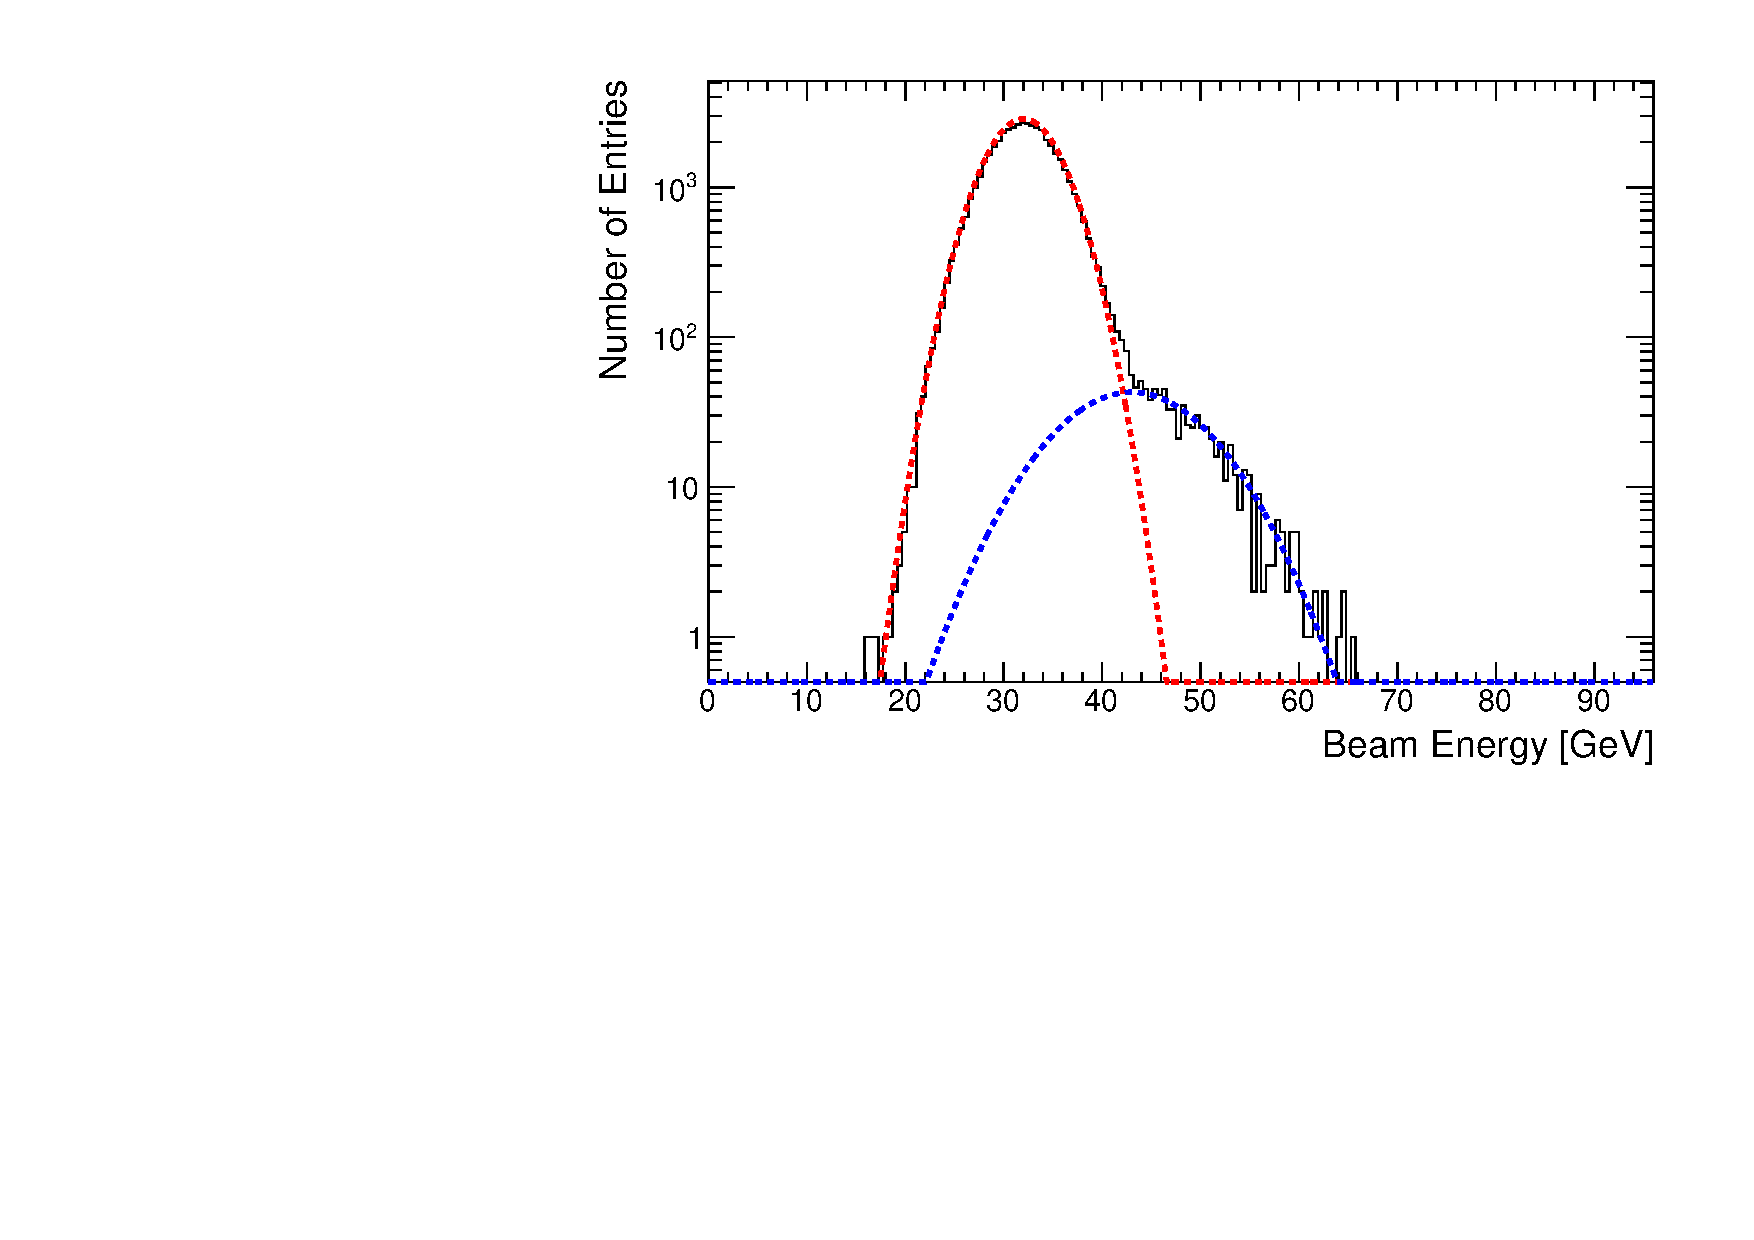
\includegraphics[width=0.8\textwidth,page=1]{toyModel}
\caption{Beam contamination toy model. The signal model function is shown in red, the contamination model (3\% amplitude) function is shown in blue. The black histogram shows 50000 random numbers drawn from the combined toy model distribution.}
\label{fig:toymodel1}
\end{center}
\end{figure}

Comparing \autoref{fig:toymodel1} and the \emph{Full Selection} in Fig. 6(a) in the current draft shows that the general shape of the resulting spectra is similar to what is left after the data selection (binning is identical, statistics are similar), although the contamination fraction is higher in this toy model than in the remaining data set. Of course the actual shape of the contamination is unknown, however the currently assumed shape is near to the worst possible case for reconstructed energy/resolution I believe.

50000 random numbers are generated according to the shape of the toy model. The resulting distribution is fitted with a Gaussian in the range of the fit applied to the actual data set (around 20-44GeV). The response and resolution are extracted from the fit and are compared to the known true values of the toy signal model. As a crosscheck also 50000 events drawn from a pure Gaussian signal distribution and fitted as well.
This whole procedure is repeated 500 times.

The deviation of the extracted response from the true response for the toy model (black curve) and the pure Gaussian signal-only model (red) is shown in \autoref{fig:toymodel2}. The deviation of the extracted response from the true response is on average around 0.3\% with width \textless 0.1\%. The deviation for a signal only model is centered around 0 with similarly small width.
\begin{figure}[htbp]
\begin{center}
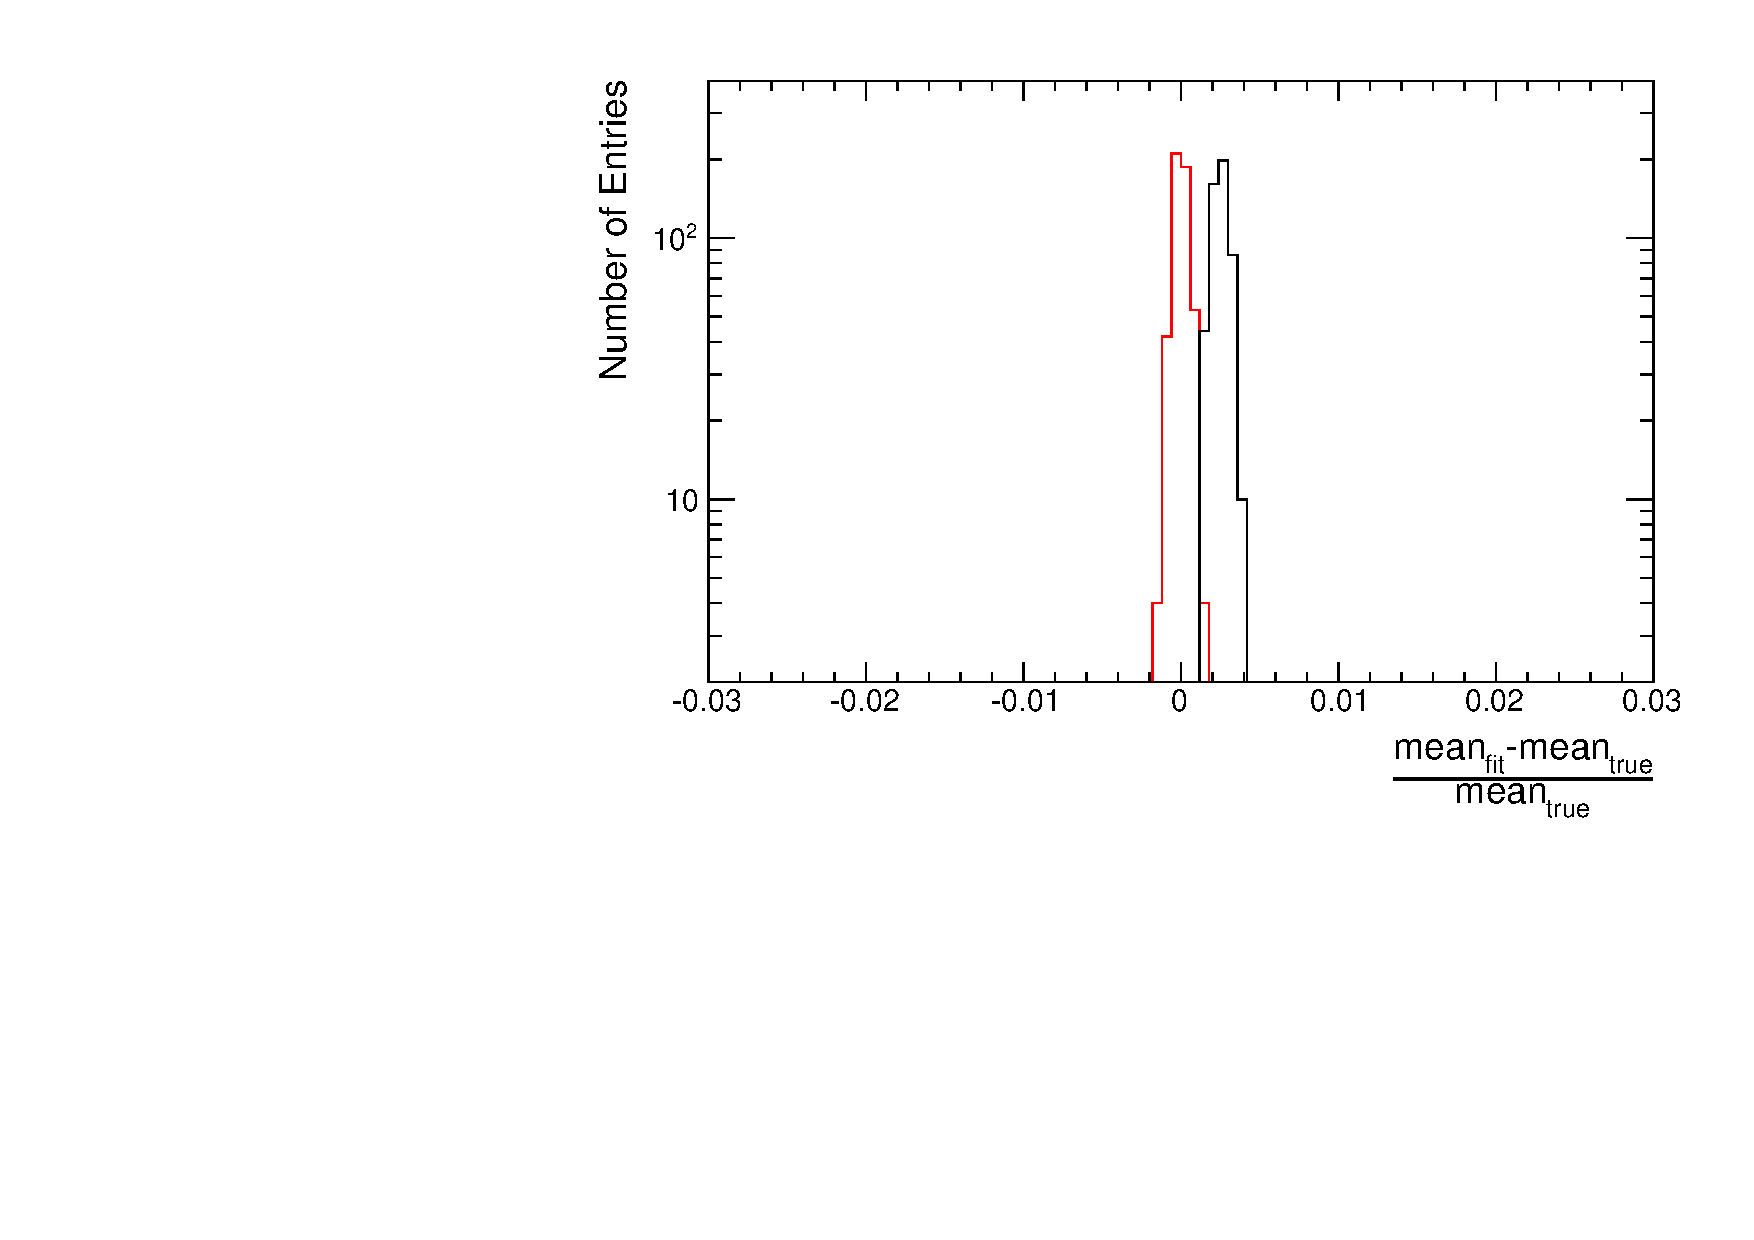
\includegraphics[width=0.8\textwidth,page=1]{ToyModelFit}
\caption{Deviation of extracted response from Gaussian fit and true response of the signal fraction of the toy model (black) and true response of a pure signal model (red). The mean of the black distribution is 0.3\%.}
\label{fig:toymodel2}
\end{center}
\end{figure} 

The same plot can be done for the extracted resolution, as shown in \autoref{fig:toymodel3}. There is a consistent overestimation of the resolution from adding the contamination model by an average of 1.8\% (relative, so 1.8\% of the 11\% resolution at 32\,GeV), which is only barely larger than the statistic fit uncertainties which are smaller than the used markers in Fig. 16(a) in the current CAN draft. Reducing the contamination fraction to a more realistic 1\% of the signal, the shift in resolution is \textless 1\%, around the same scale as the statistical uncertainties.
\begin{figure}[htbp]
\begin{center}
\includegraphics[width=0.8\textwidth,page=3]{ToyModelFit}
\caption{Deviation of extracted resolution from Gaussian fit and true resolution of the signal fraction of the toy model (black) and true resolution of a pure signal model (red). The mean of the black distribution is 1.8\%.}
\label{fig:toymodel3}
\end{center}
\end{figure} 

I propose not to include this systematics study into the CAN, as I feel it is already rather too long. I added a sentence stating that the systematic uncertainties on response and resolution from the remaining contamination are small in ll. 214--215 of the updated draft.
\clearpage
\begin{quote}\texttt{Line 309, because of superior performance the hit energy rather than hit density is used for the software compensation.  How big is the effect from this change and can you explain this behavior?}\end{quote}
I do not have the exact numbers on hand, but I remember it was less than 1\% (absolute) decrease in resolution for each energy point. For the explanation of this behaviour I again quote my answer to Daniel's very similar question:

``Measuring a deposition of around 1MIP is in the very most cases exactly one traversing particle (disregarding downward fluctuations from the Landau and photon statistics). No single particle can deposit less than that energy (apart from very low energy particles that get stuck and deposit all their remaining kinetic energy in a tile). So for depositions around 1 MIP, dividing by the tile area for density does not really make sense, as we know the deposition is not distributed over the tile surface but most likely came from a single particle. Most of all hits are around the single MIP level anyway, even more so in the outer parts of the AHCAL, as shown in \autoref{fig:hitenergies_inner_outer} (please excuse the ugly quick and dirty plot).
\begin{figure}[htbp]
\begin{center}
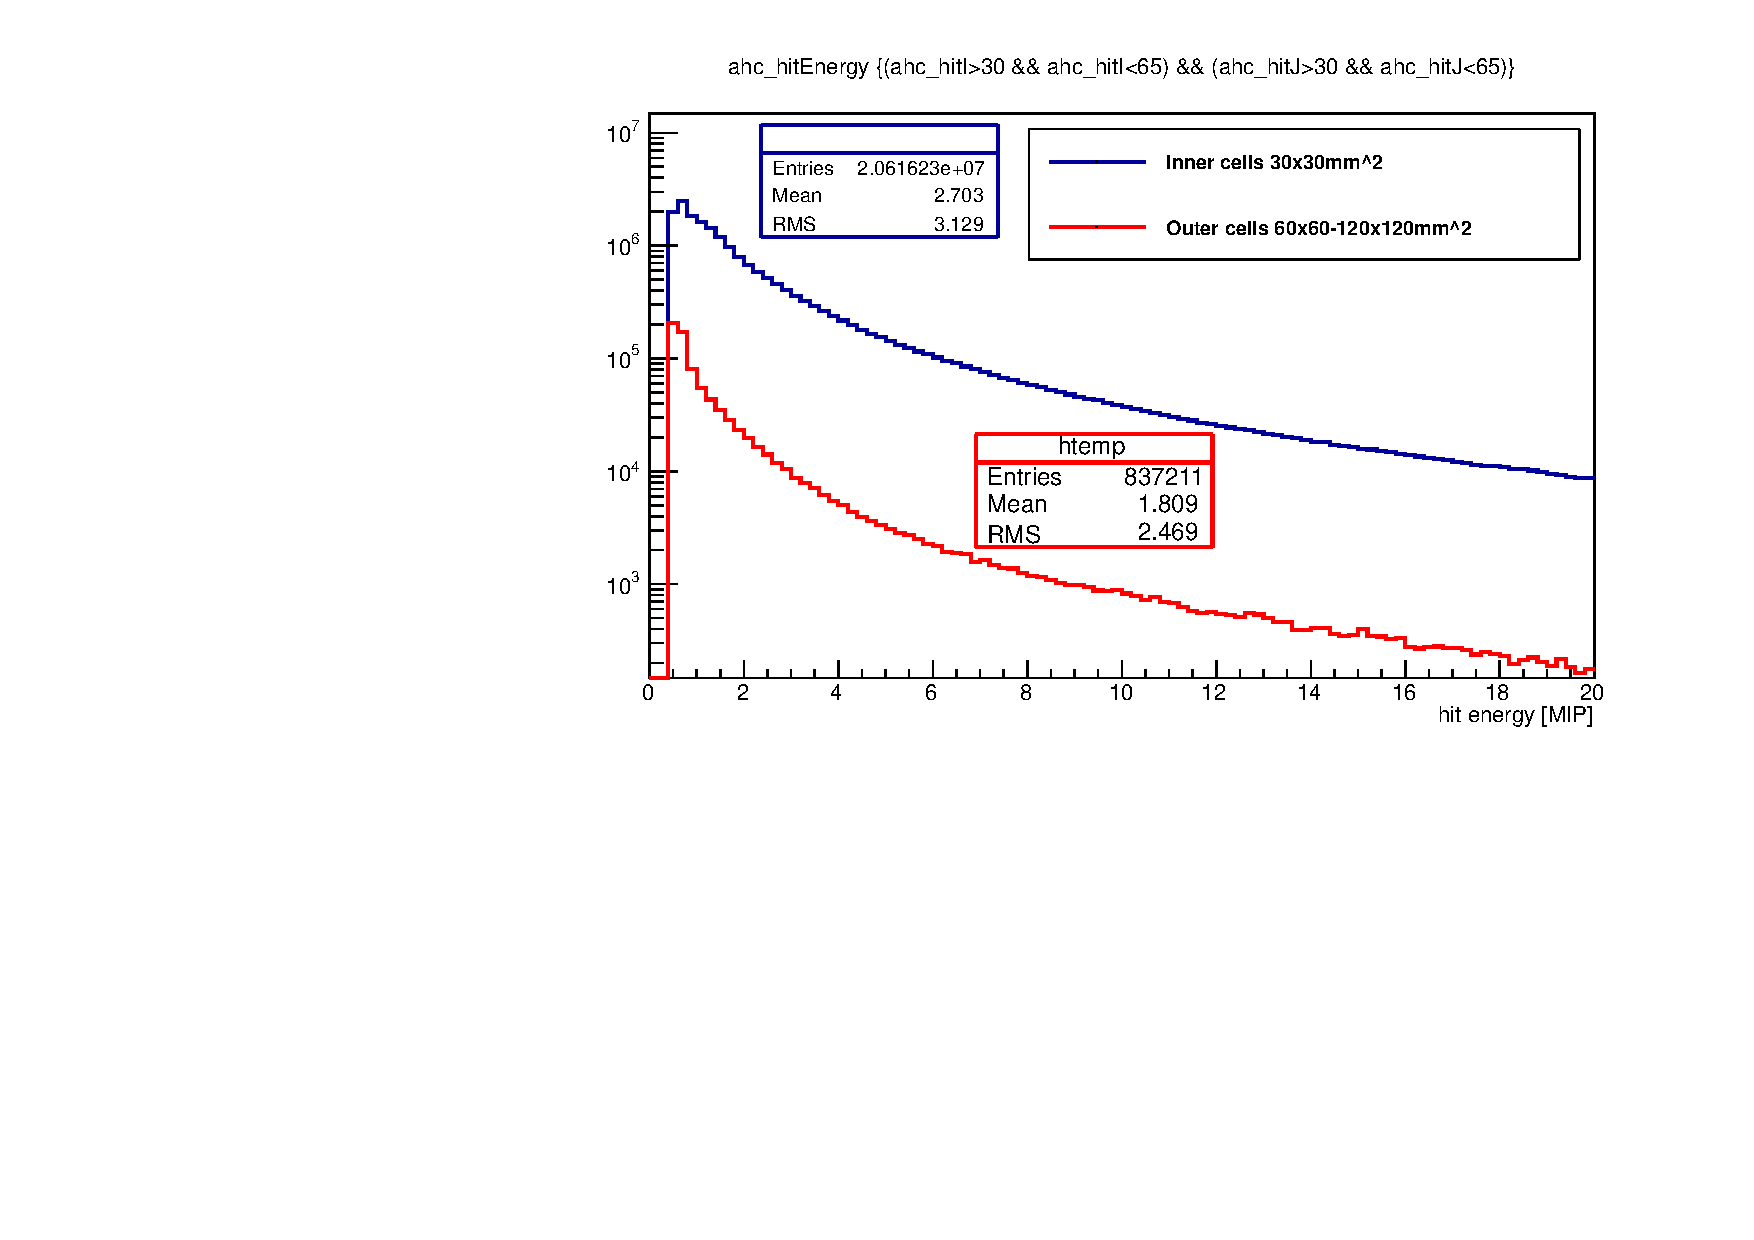
\includegraphics[width=0.7\textwidth,page=1]{hitenergy_AHCAL_inner_vs_outer_cells_560474_MC}
\caption{AHCAL Hit energy distribution of the central, finely segmented core of 30*30mm\textsuperscript{2} tiles and the outer, coarser rings of 60*60 to 120*120\textsuperscript{2} tiles.}
\label{fig:hitenergies_inner_outer}
\end{center}
\end{figure}
 When using the true measured deposition density instead of the hit energy, most energy depositions of the larger AHCAL cells will fall into the first two hit energy bins (0.5-2MIP), which is also not really what we want to do. Ideally one would have separate software compensation weights for each tile size. In practice there is not enough statistics in these cells to do that, and the number of parameters and computation time in optimisation would increase by an unreasonable amount.''

\begin{quote}\texttt{Line 317, does the TCMT help at all?  What happens if it is omitted?}\end{quote}
It helps the energy resolution significantly at 32\,GeV. The increase in leakage (in shape of the low-energy tail in the reconstructed energy spectrum) when excluding the TCMT is visible by eye in \autoref{fig:tcmt_comp_32gev}. Also for lower energies down to 12\,GeV the TCMT significantly improves the energy resolution, albeit absolutely and relatively less. A summary of standard reconstruction energy resolutions with and without TCMT is given in \autoref{table:tcmt_reso}. The granularity (and in general calibration and noise profile) of the TCMT is not sufficient to effectively use software compensation techniques, so all TCMT compositions are weighted with one energy-parametrised weight. In practice it would make no difference to assign an energy-constant weight for all TCMT depositions also in software compensation reconstruction. The main reason the TCMT is included in this analysis is to be able to compare directly to the published AHCAL+TCMT energy resolution as shown in Fig.17 (Fig.18 in the updated draft).
\begin{figure}[htbp]
\begin{center}
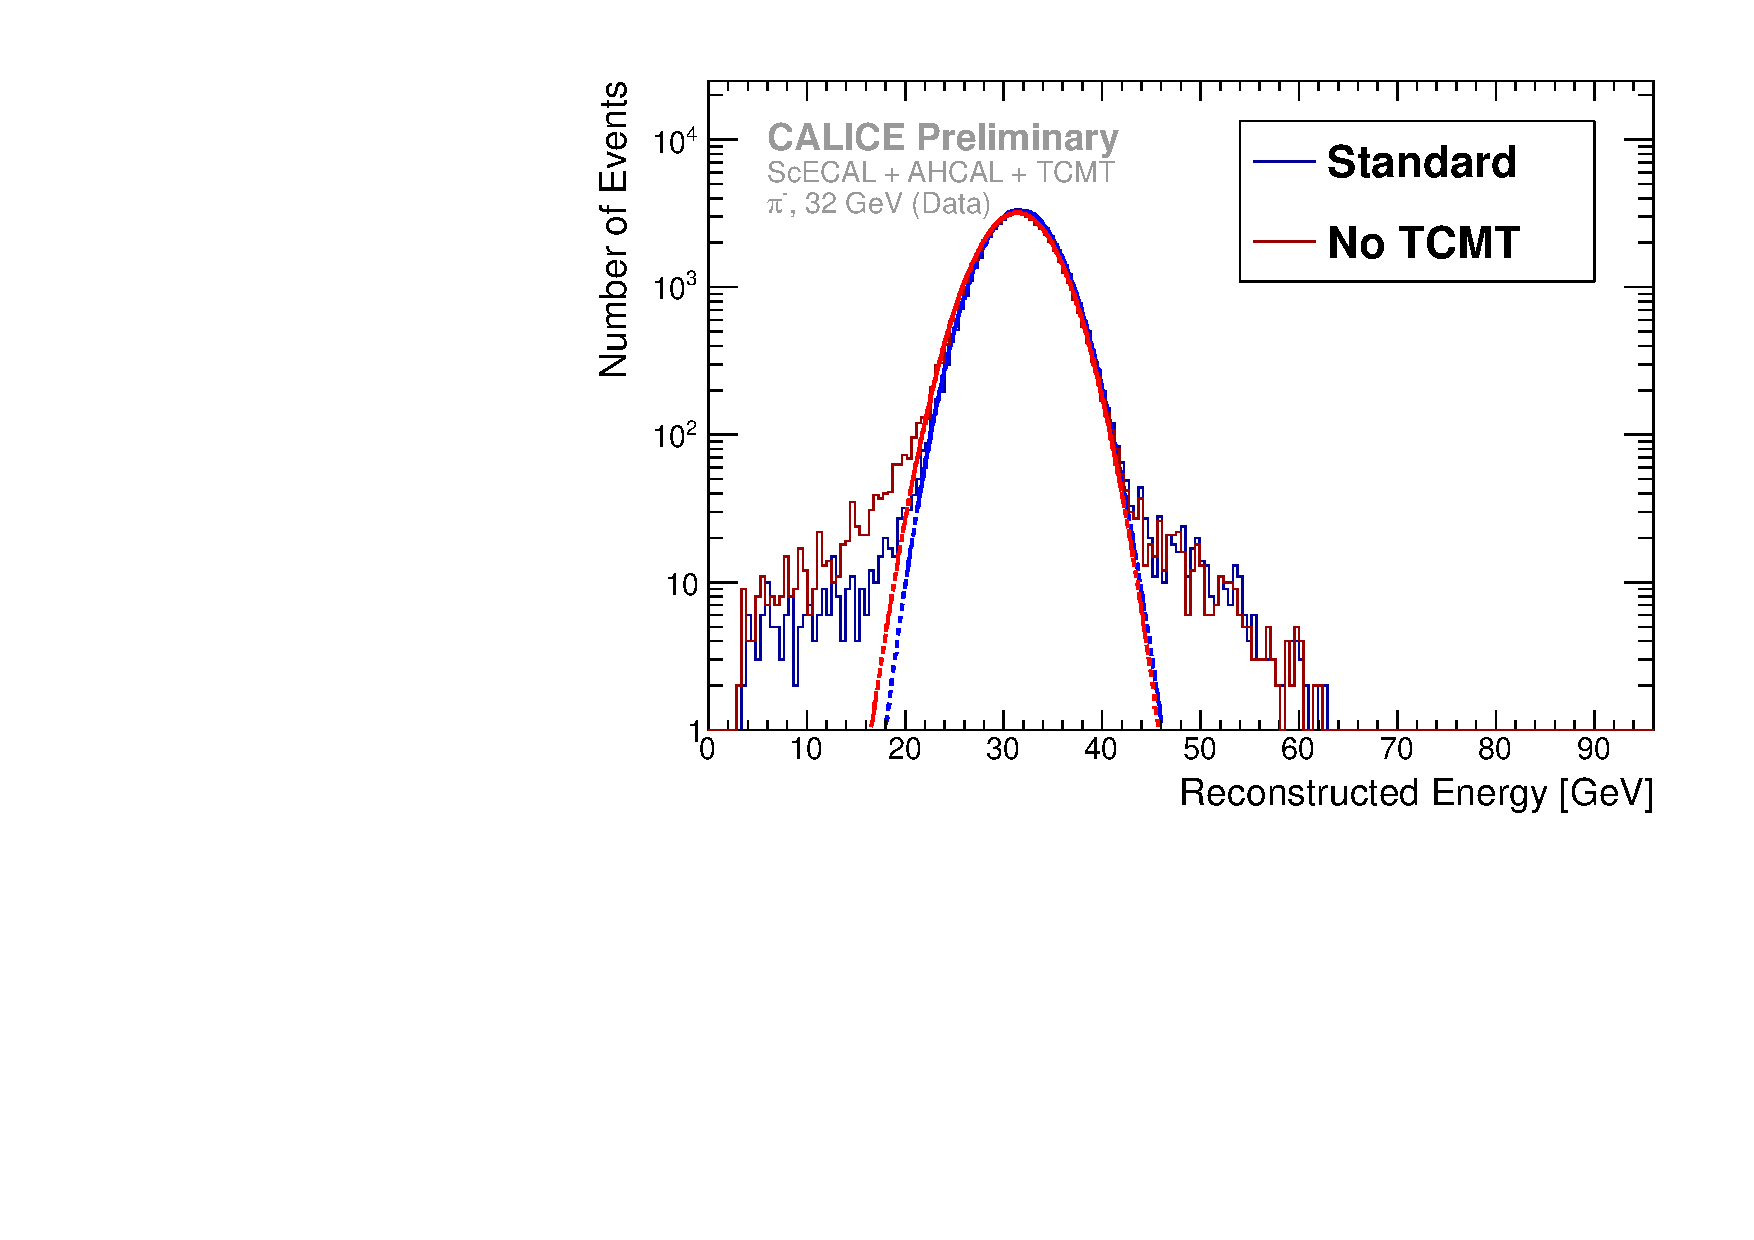
\includegraphics[width=0.7\textwidth]{ERec_classic_noTCMT_560474_data}
\caption{Reconstructed hit energy spectrum of data run 560474 (32\,GeV \piminus) in standard reconstruction with and without TCMT depositions.}
\label{fig:tcmt_comp_32gev}
\end{center}
\end{figure}

\begin{table}[htbp]
\begin{center}
\caption{Standard reconstructed energy resolutions with and without incorporating depositions in the first 8 layers of the TCMT. The resolutions at 4\,GeV are consistent within the statistical fitting uncertainties.}
\label{table:tcmt_reso}
\begin{tabular}{lll}
energy [GeV]	&	w/ TCMT & w/o TCMT \\\hline
4		&23.3\%		& 23.6\% \\
12		&16.0\%		& 16.3\% \\
15		&14.6\%		& 14.9\% \\
20		&13.0\%		& 13.4\% \\
32		&10.8\%		& 11.4\% \\
\end{tabular}
\end{center}
\end{table}

\begin{quote}\texttt{Equation 3, can you please provide an explanation as to how this formula suppresses fluctuations? For example how would it treat a pion shower that went mostly electromagnetic or mostly hadronic?}\end{quote}
The general idea of software compensation and the approach taken here is explained in ll.290--300 of the draft, while the concrete implementation leading to Equation 3 is explained in ll.300--318. The correlation plot in Fig 10(b), explained in ll.348--350, gives an example of the working mechanism of the software compensation implemented here, however it is very short. I have extended the explanation about Fig. 10(b) in the updated draft, now including explicit explanations for the behaviour in hadronic-heavy and EM-heavy hadron showers in ll.351--357 of the updated draft.
 
\begin{quote}\texttt{Equation 3, was all the data used to find the weights?  How do the weights vary with the training sample size?}\end{quote}
This is mentioned in line 250 of the draft, the first 40k events of each data run (first 20k events in MC) are used in the optimisation. There is no significant difference in the reconstructed energy and resolution of the data sample that has been used for parameter optimisation and the part of the data sample that has not been used for parameter optimisation. Thus all events are included in the analysis to preserve statistics. I have extended the sentence in ll.251--252 to reflect that it relates to both standard and SC reconstruction. The weights obtained from randomised optimisation event samples vary within the statistic uncertainties given by the optimisation as shown in the error bands of Fig. 11.

\begin{quote}\texttt{In Figs. 9c and 9d why are the lower bin weights slanted lines?  Rather than just levels as with the other higher energy bins?  (sorry if I missed this in the text)}\end{quote}
This is mentioned in the second to last sentence of the description of Fig 9. The slanted bin weight corresponds to a $a\times\nicefrac{1}{E}$ dependence, which exactly equals a counting of each hit in that bin with weight $a$. Most people are confused about this initially, so I agree this needs more clarification in the text. I have added one more sentence about the sloped bin weights in the text in ll.339--341 of the updated draft.

\begin{quote}\texttt{The data/simulation weight differences in the first and last bins are interesting.  How dependent is the resolution on these weights?  Perhaps there is just no sensitivity.  As a test, what happens when these weights are altered arbirtrary by 25 and 50\%}\end{quote}
Just to clarify: Only the ScECAL SC weights are affected from this, the AHCAL SC weights are very similar between data and MC in all bins.
 
Generally if there was no sensitivity, switching from weighting bins to counting bins in the first two bins would not help at all (discrepancies in data/MC weights stay similar when disabling the counting in the first bins). Most depositions (by number of hits) are in the first bins (see \autoref{fig:hitenergies_inner_outer}), however most depositions by energy sum are neither in the first nor last bin (see Fig. 12(a),(c) in the CAN draft). This is also supported by the obtained uncertainties from the parameter optimisation. A bin weight that has no (or small) influence on the overall resolution will show an increased uncertainty band. This can be clearly seen in Fig.9(d) of the draft, where the weight uncertainty for the highest AHCAL hit energy at 4\,GeV beam energy (blue curve, last bin) has a much larger uncertainty than the other bins, because there is practically no deposition in this bin at 4\,GeV (see also the last bin in Fig 12(b)).

For reference I have included the SC parameter correlations between hit energy bins, as extracted from the Minuit optimisation, in \autoref{fig:correlations}. Neighboring bins are typically anti-correlated (if at all). Indeed the SC weight of the first bin is higher in MC than in data, and the lower in MC than in data in the second bin. Thus forcing down the optimised SC weights of the first bin and rerunning the optimisation would definitely lead to more similar weights in data and MC. In addition to the updated draft I will upload a document weightsSC.pdf which includes all optimised SC weights in data and MC for ScECAL, AHCAL and TCMT if you are interested.
\begin{figure}[htbp]
	\subfigure[Data] {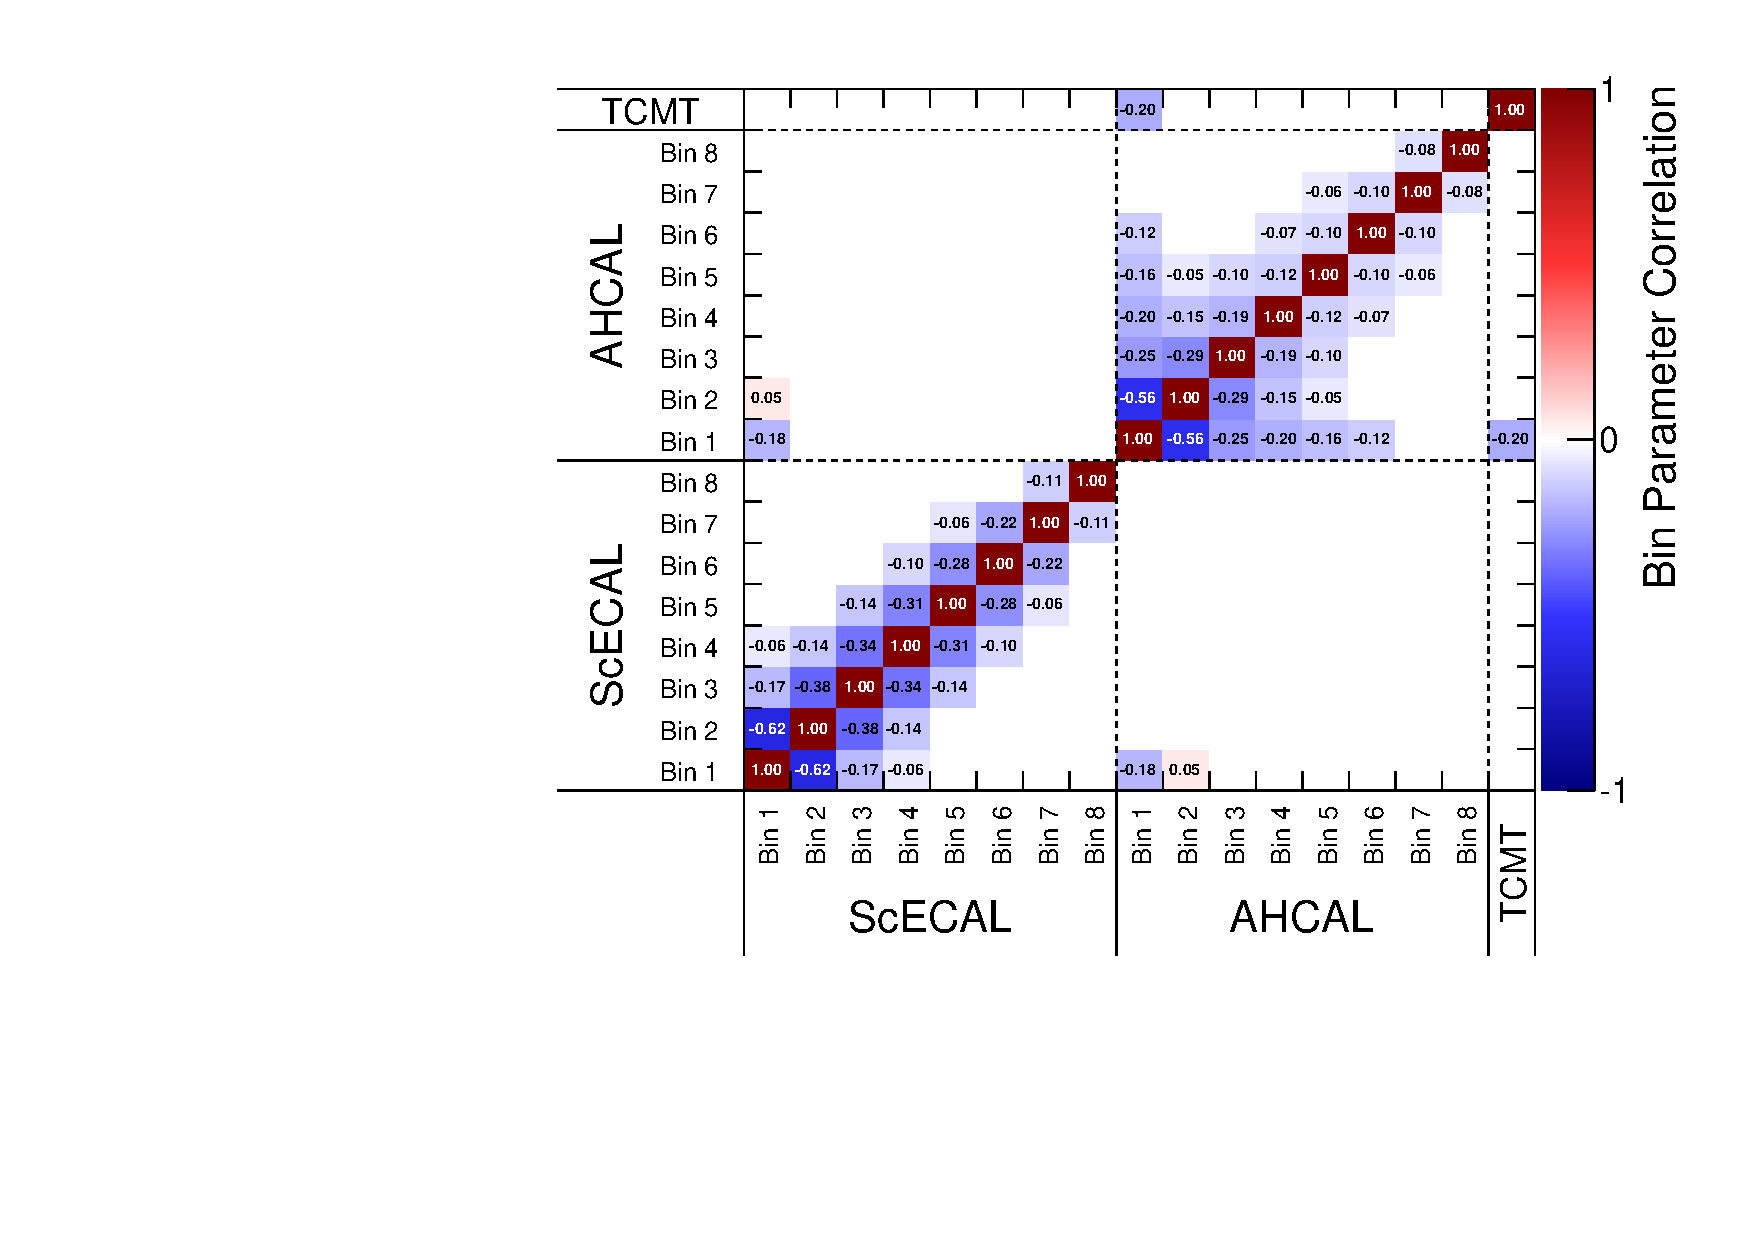
\includegraphics[width=0.80\textwidth]{paramCorrelation_DATA}}\hfill
	\subfigure[MC QGSP\_BERT\_HP (G4 10.1p2)] {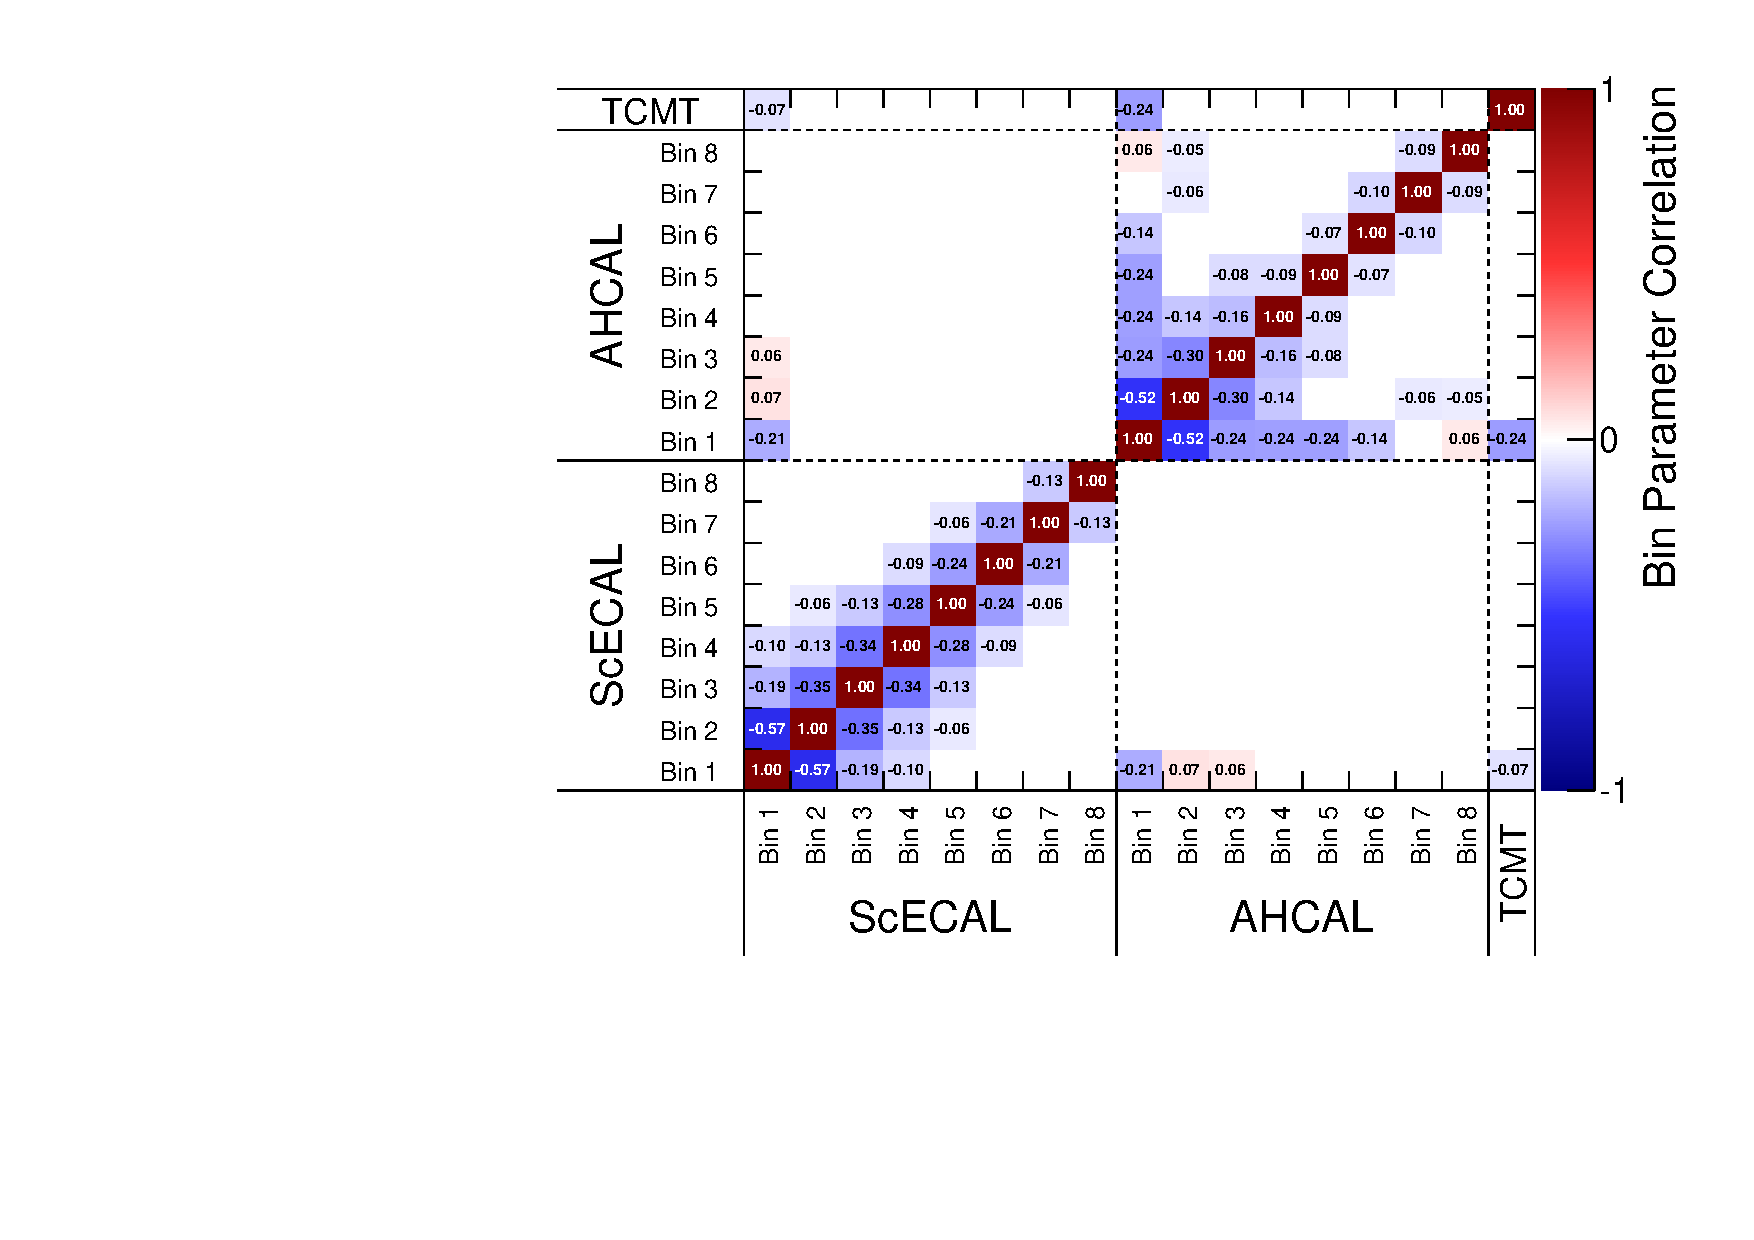
\includegraphics[width=0.80\textwidth]{paramCorrelation_QGSP_BERT_HP}}
	
	\caption[]{Parameter correlations for software compensation bin weights extracted from the Minuit parameter optimisation. Observed correlations are up to 10\% smaller in simulation, but the general ``shape'' of correlations is identical.}
	\label{fig:correlations}
\end{figure} 

Randomly shifting weights would certainly deteriorate the reconstructed energy response. Instead, to get an idea of the influence of the SC weights, I have reconstructed the data sample using the SC weights from simulation. (As the SC weights are multiplied on top of the standard weights, I use the standard weights from data and the SC weights from QGSP\_BERT\_HP in G4 10.1p2). This was also obviously (possibly suspiciously) missing from the note before.

 The table showing reconstructed mean energy and reconstructed resolution is given in \autoref{table:sc_data_mc}. Applying the SC weights from MC to data seems to slightly improve the energy resolution of most energy points (1--3\% relative), for the price of a slightly worse response reconstruction (also in the range 1--4\% relative). I hope this clarifies your question.

I have added two paragraphs and two new plots to the note, showing and discussing the results obtained when SC weights from MC are applied to data in ll.467--484 of the updated draft.
\begin{table}[htbp]
\begin{center}
\caption{Response and resolution of data runs, reconstructed with SC weights optimised from data and SC weights optimised from QGSP\_BERT\_HP simulation samples.}
\label{table:sc_data_mc}
\begin{tabular}{lllll}
energy 	&reso (data w.)	&resolution (mc w.)	&response (data w.)	&response (mc w.) \\\hline
4\,GeV		&21.2\%				& 20.6\% 		&	4.00\,GeV	& 4.14\,GeV	\\
12\,GeV		&14.4\%				& 14.1\% 		&	11.7\,GeV	& 11.7\,GeV	\\
15\,GeV		&12.8\%				& 12.6\% 		&	14.7\,GeV	& 14.6\,GeV	\\
20\,GeV		&11.0\%				& 10.9\% 		&	19.9\,GeV	& 19.7\,GeV	\\
32\,GeV		&8.4\%				& 8.4\% 		&	31.8\,GeV	& 31.3\,GeV	\\
\end{tabular}
\end{center}
\end{table}


\begin{quote}\texttt{Figure 15, is there any understanding as to why the SC response is the worst  at 12 GeV?  Is this some sort of statistical bias? Is the data set compromised somehow?   Could we please see the resolution plots and fits for the data at all points?}\end{quote}
I do not know for sure. There is no statistical bias between runs, as each run is using the same number of events (40k in data, 20k in MC) for optimising the weights. However there is some inherent biasing because of the distribution of runs in energy (assume we would have runs at 1, 2, 3, 4, and 32\,GeV, even when using the same statistics in each run the 32\,GeV run would probably reconstruct worse as the optimisation will favor the lower energy par). Assuming that hadronic interactions show a different behaviour at 4\,GeV and 12+\,GeV (e.g. in MC the mean number of secondary particles produced in the first inelastic hadronic interaction is much higher at 4\,GeV than at 12\,GeV and upwards! I don't know if this is also seen in real life or just an effect of switching between different parametrisations in MC in that energy range though), the fact that there is no energy points in between 4\,GeV and 12\,GeV somehow causes a hard transistion. There are not enough degrees of freedom in the parametrisation (every weight is a 2nd order polynomial as a function of the beam/reconstructed energy) for a hard step, so the optimisation optimises the overall $\chi^2$. As the behaviour is the same in data and MC (at least in the SC case) I do not believe the dataset is compromised.

All data runs with fits (in standard and SC reconstruction) are shown at the end of this document. Do you think I should add these plots into the appendix of the CAN?

In addition to the changes to the draft discussed to the text, following comments from Jose during the recent CALICE meeting in Fukuoka, I have updated the x-axis titles of Figs. 9(a),(b) and 11 to reflect that during reconstruction only the standard reconstructed particle energy is used to lookup the appropriate SC weights for each event. 

I have uploaded a the new draft v1.2, this document and the collection of SC weight plots to the INDICO.

Cheers,
Oskar


\clearpage
\begin{figure}[htbp]
\begin{center}
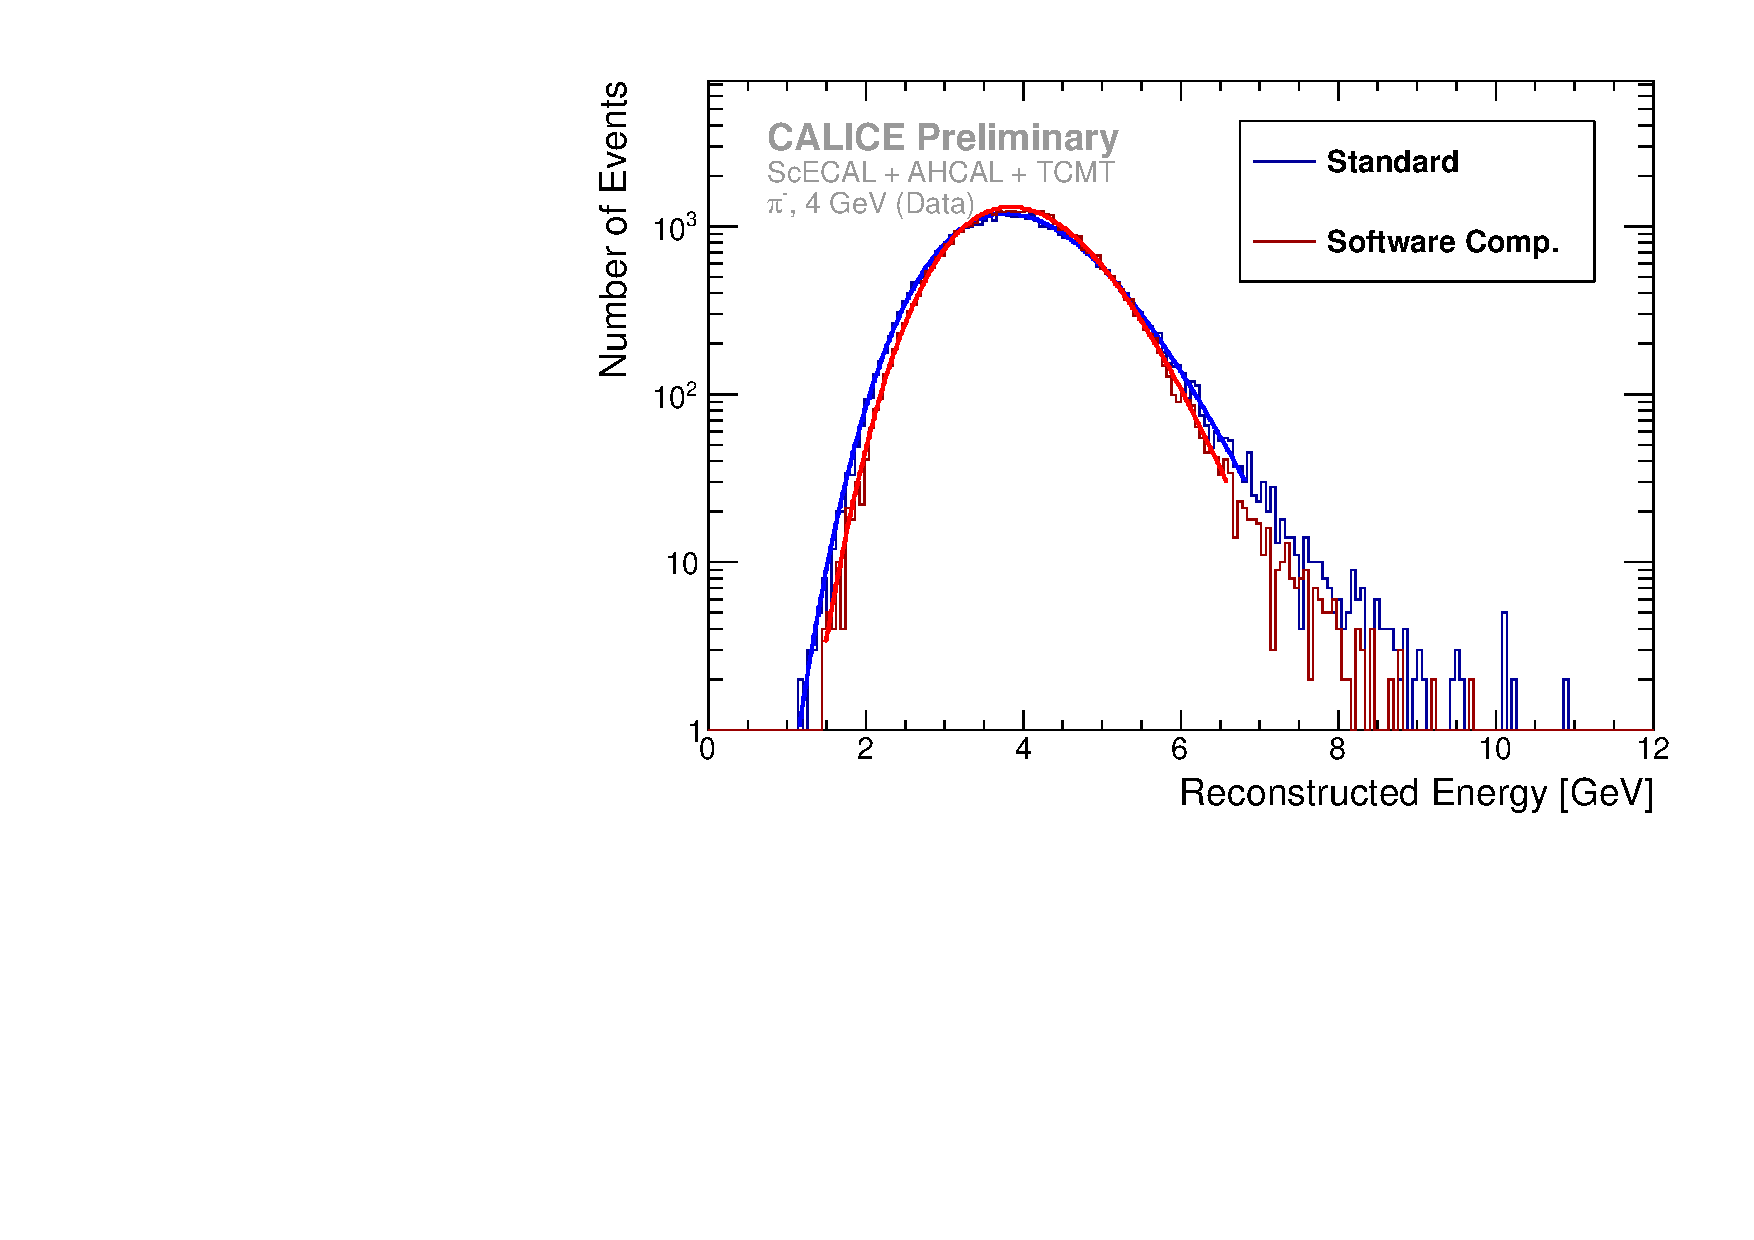
\includegraphics[width=1\textwidth,page=1]{ERec_classic_SC_560506_data}
\caption{Reconstructed energy for Run 560506, 4\,GeV \piminus.}
\label{fig:erec_4gev}
\end{center}
\end{figure}

\begin{figure}[htbp]
\begin{center}
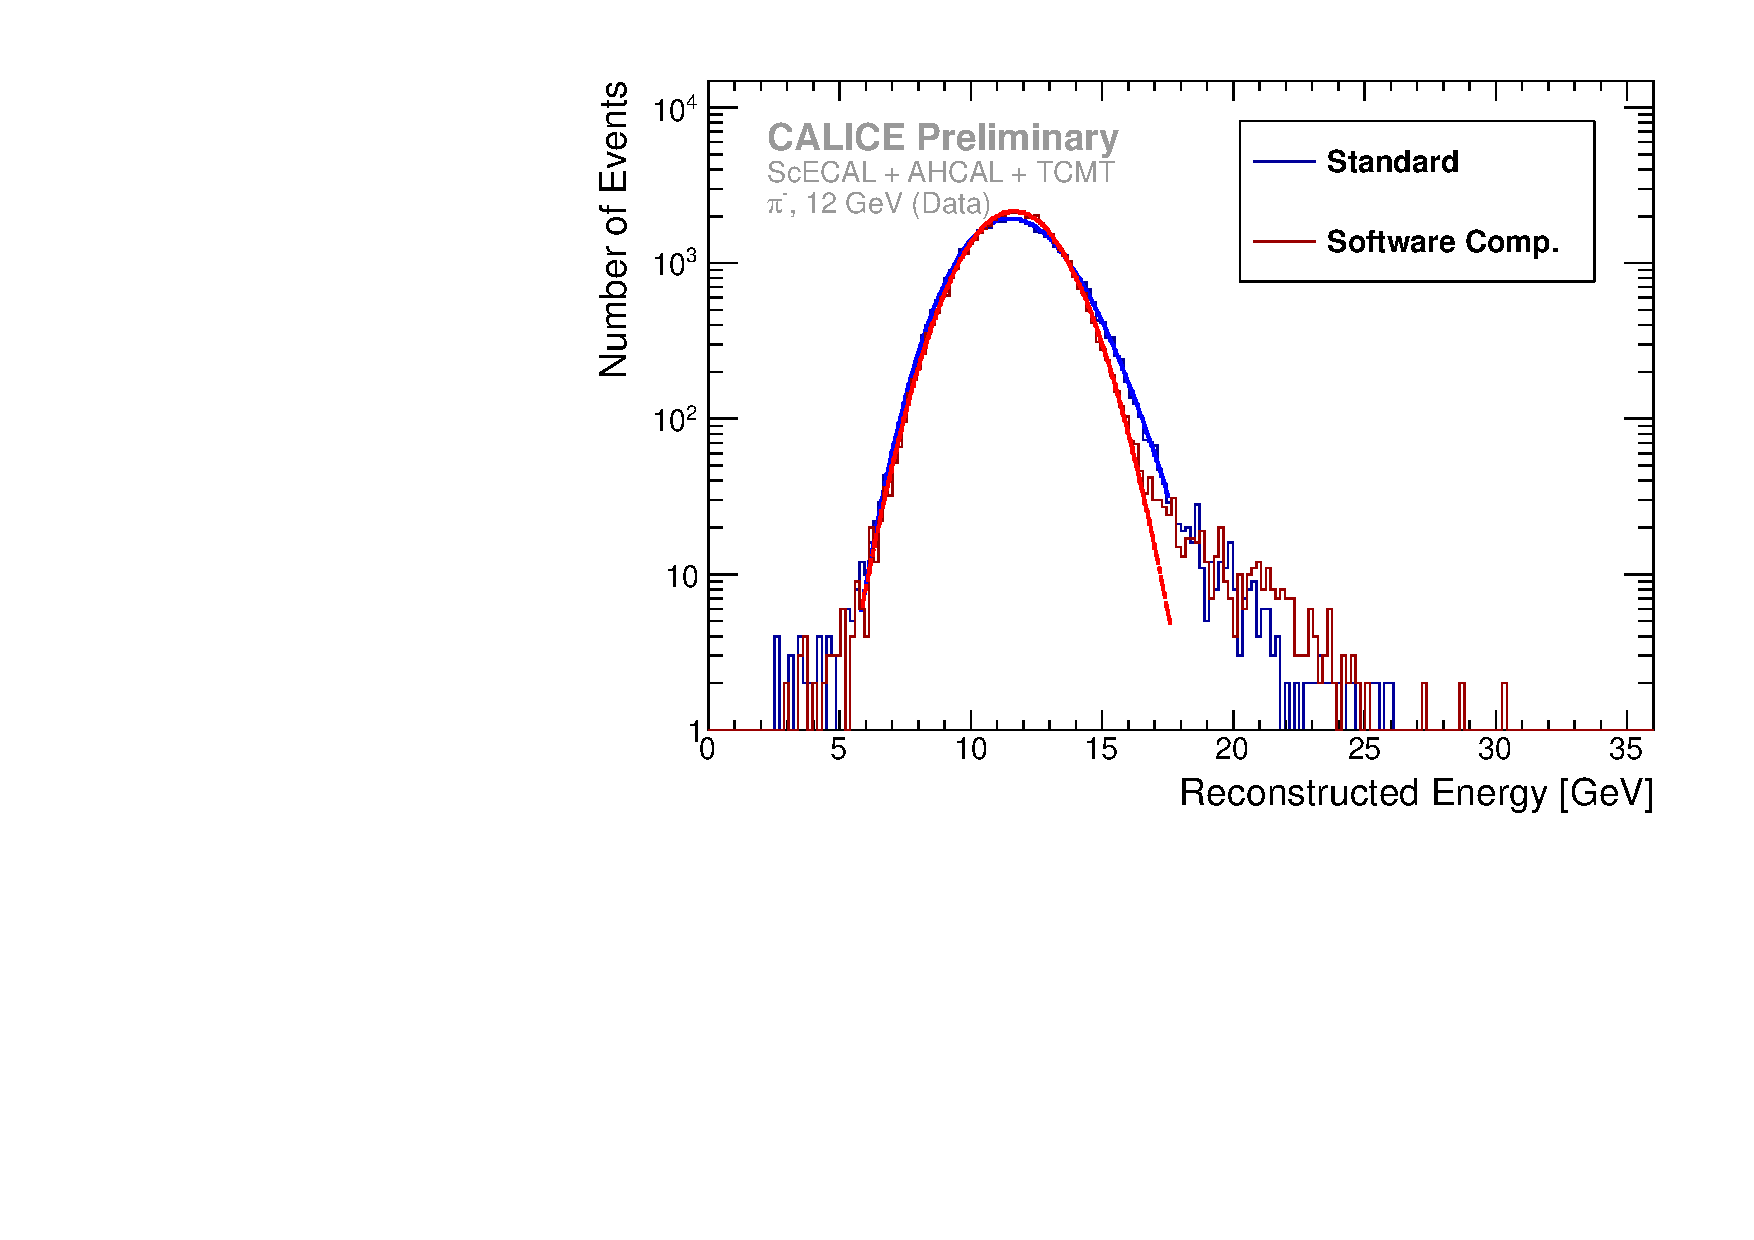
\includegraphics[width=1\textwidth,page=1]{ERec_classic_SC_560498_data}
\caption{Reconstructed energy for Run 560498, 12\,GeV \piminus.}
\label{fig:erec_12gev}
\end{center}
\end{figure}

\begin{figure}[htbp]
\begin{center}
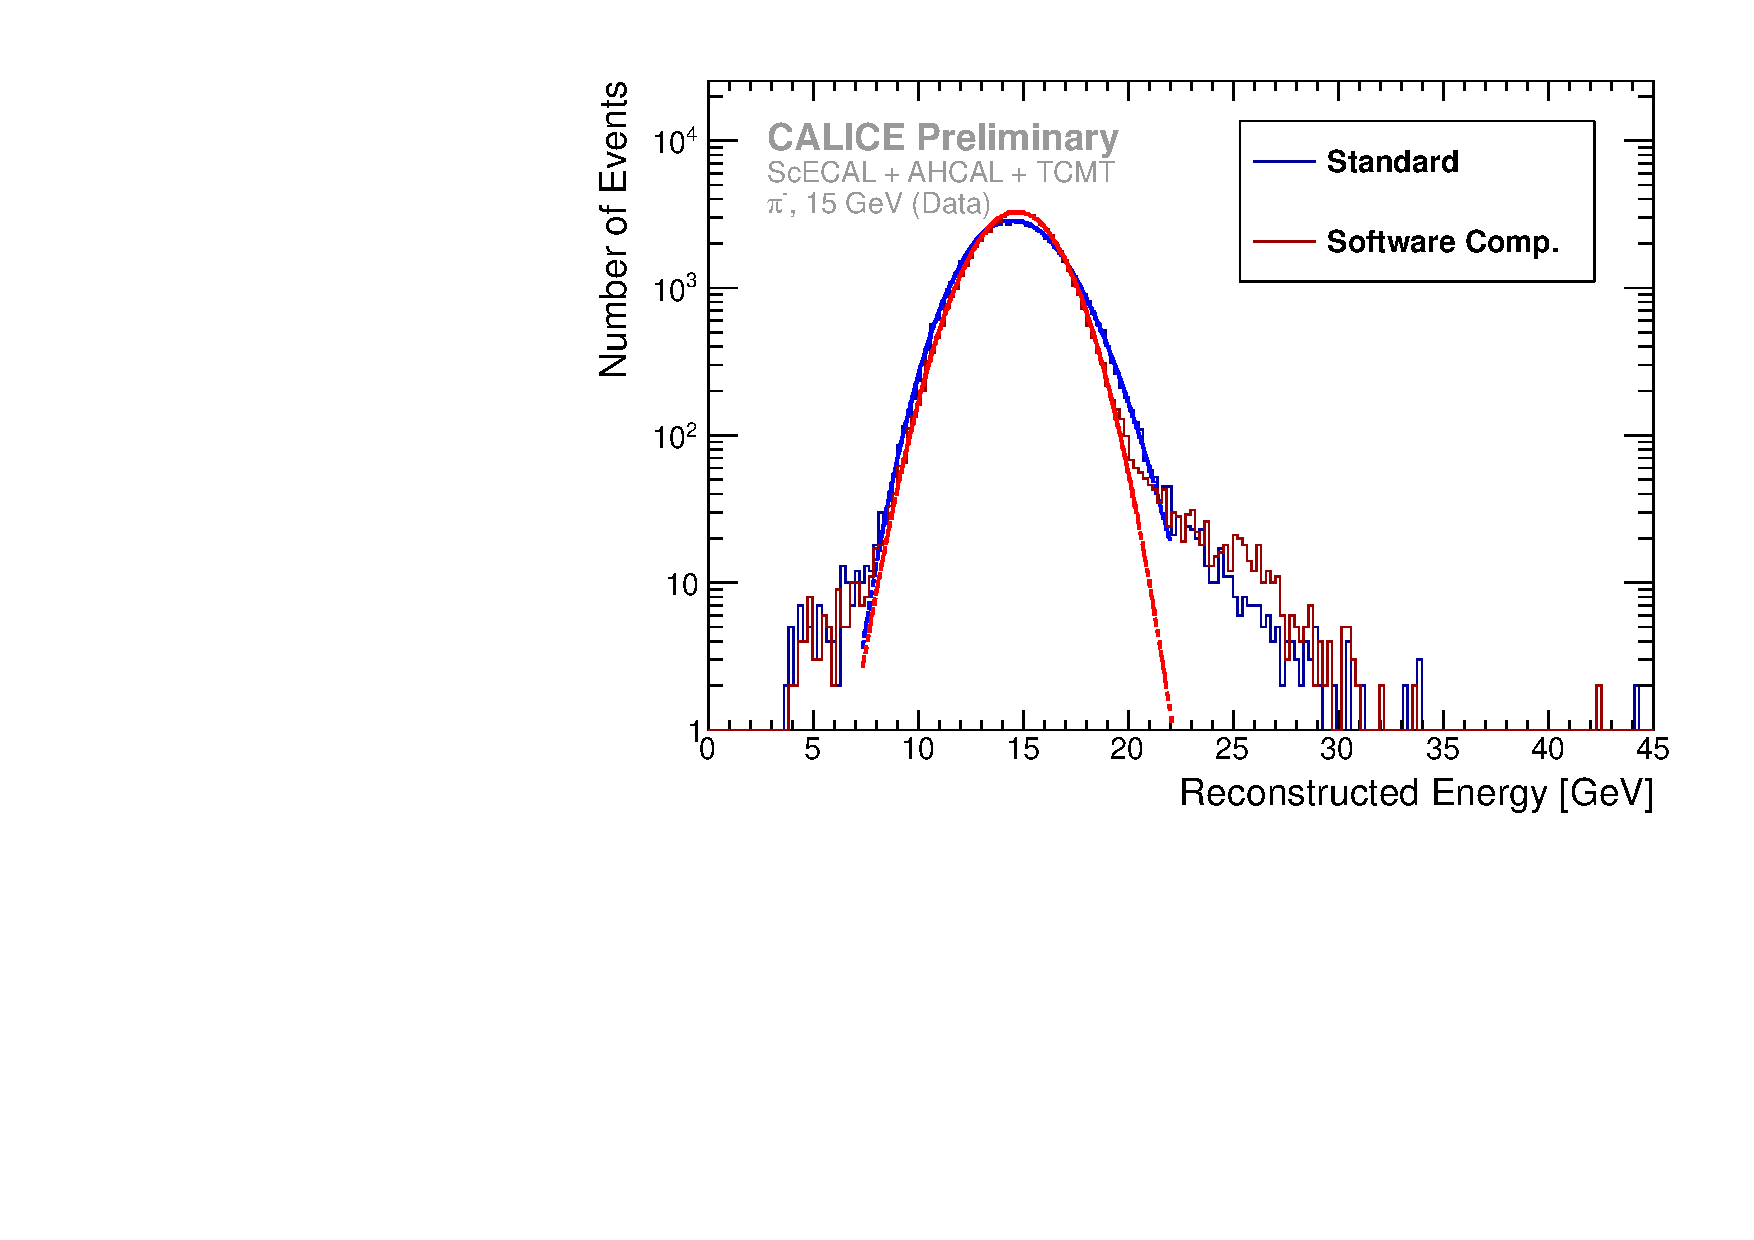
\includegraphics[width=1\textwidth,page=1]{ERec_classic_SC_560496_data}
\caption{Reconstructed energy for Run 560496, 15\,GeV \piminus.}
\label{fig:erec_15gev}
\end{center}
\end{figure}

\begin{figure}[htbp]
\begin{center}
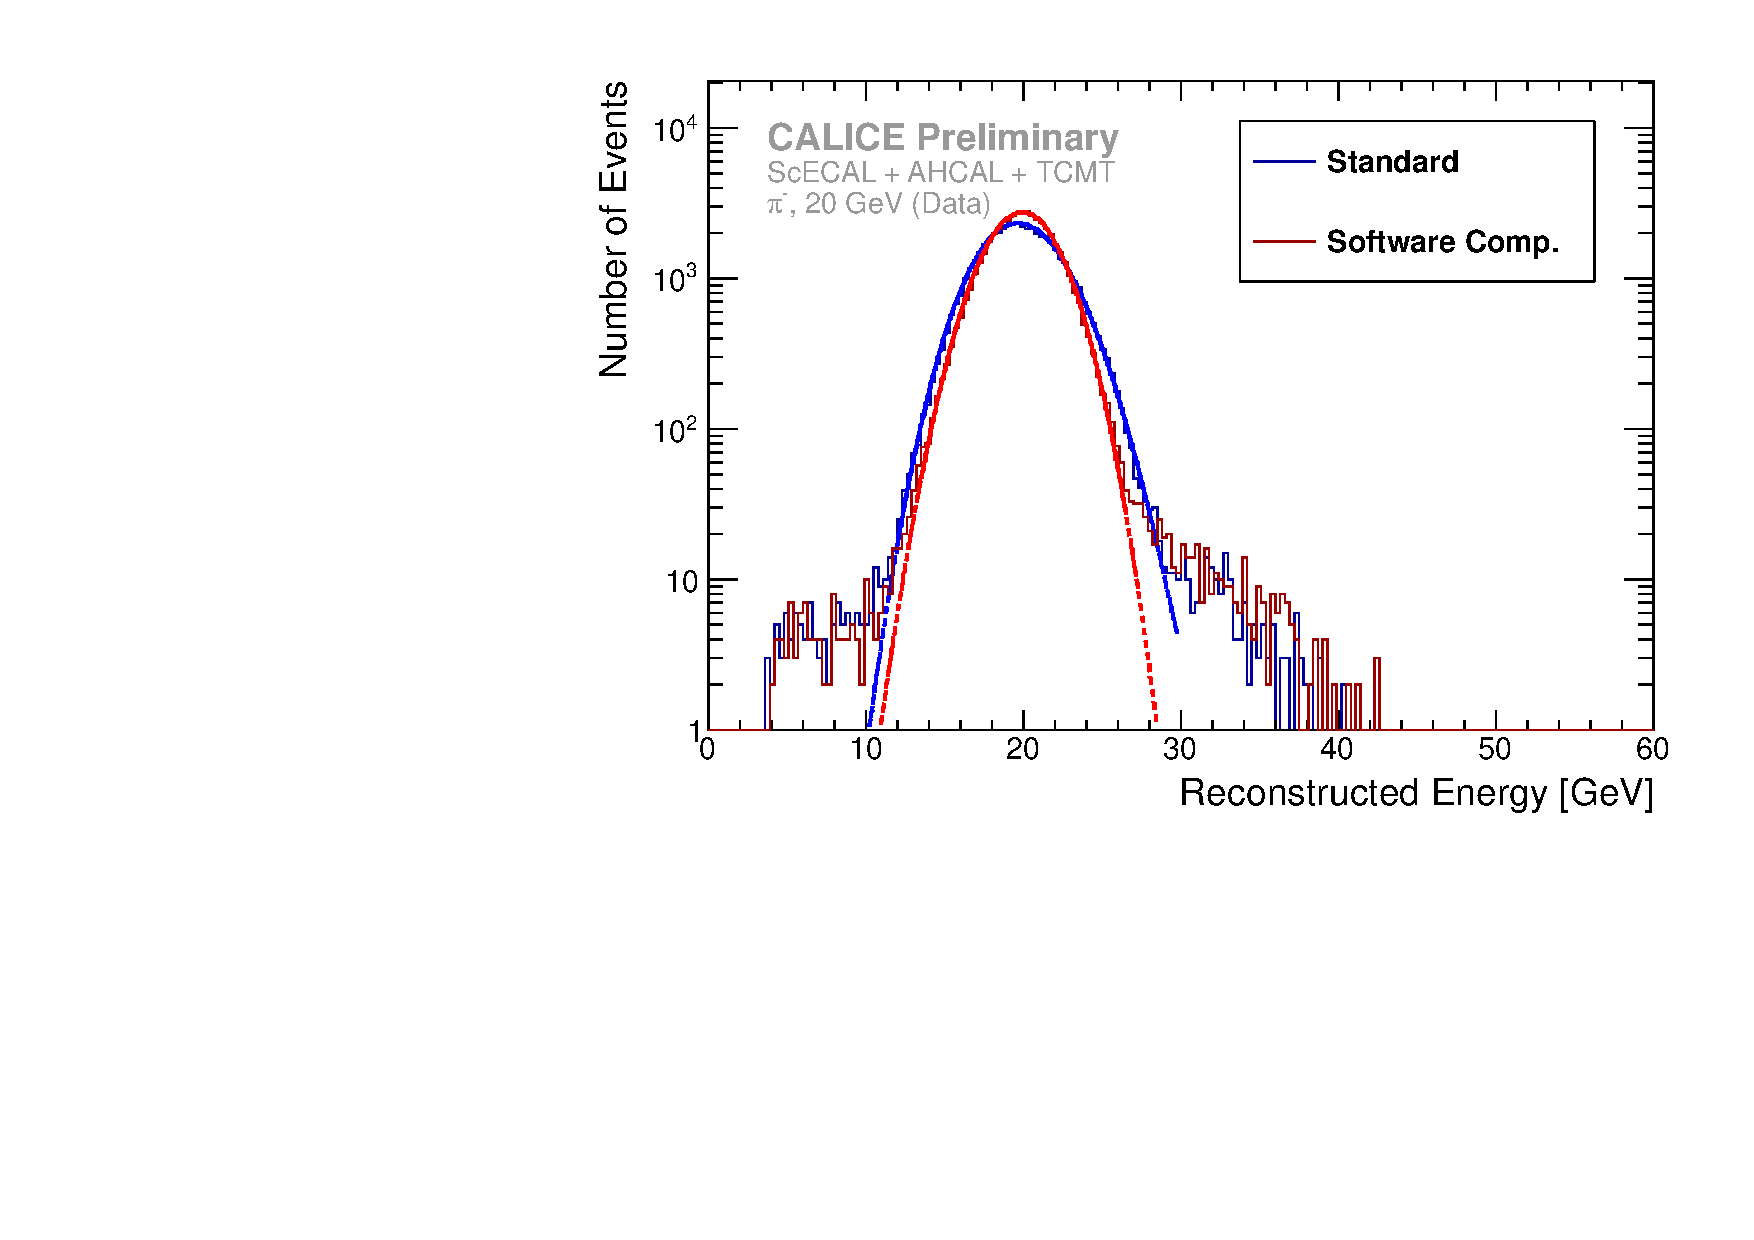
\includegraphics[width=1\textwidth,page=1]{ERec_classic_SC_560481_data}
\caption{Reconstructed energy for Run 560481, 20\,GeV \piminus.}
\label{fig:erec_20gev}
\end{center}
\end{figure}

\begin{figure}[htbp]
\begin{center}
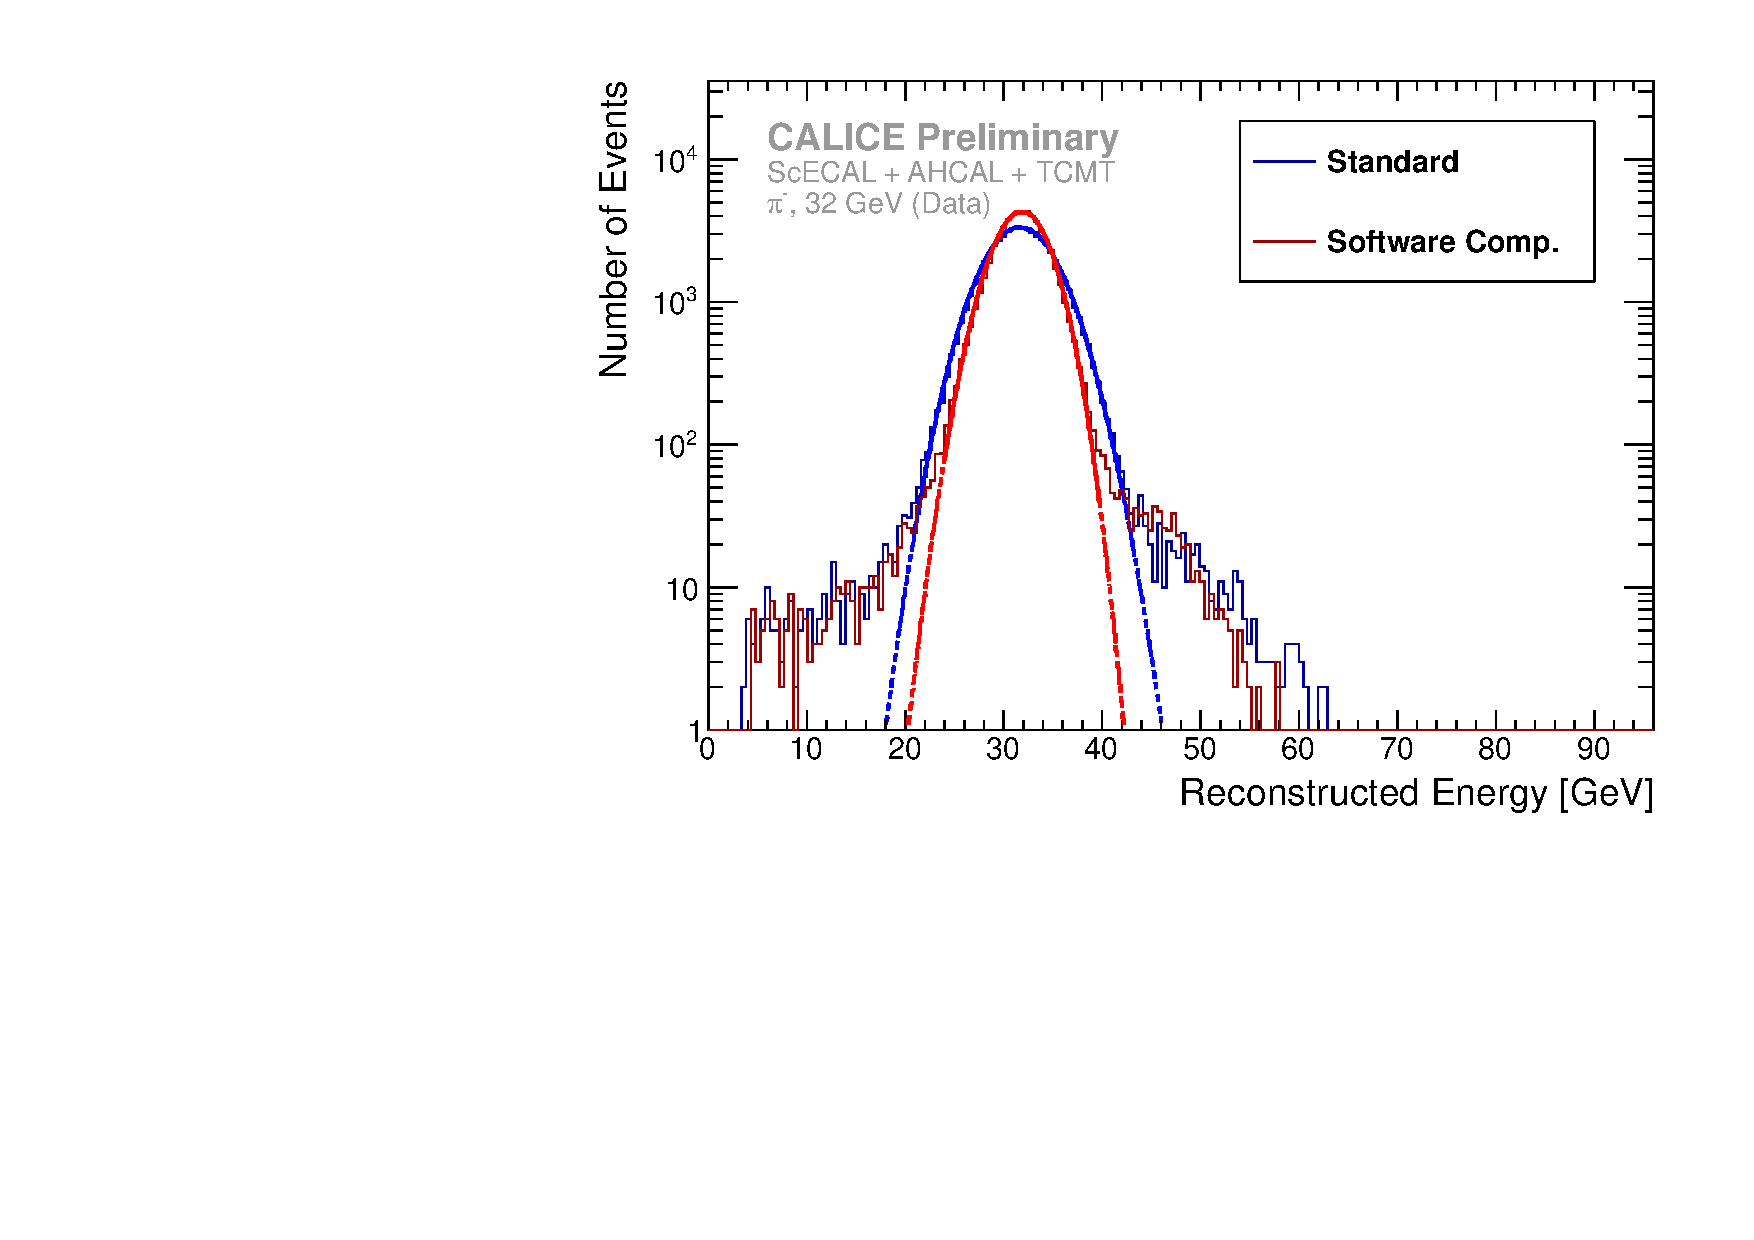
\includegraphics[width=1\textwidth,page=1]{ERec_classic_SC_560474_data}
\caption{Reconstructed energy for Run 560474, 32\,GeV \piminus.}
\label{fig:erec_32gev}
\end{center}
\end{figure}


\end{document}
